% *******************************************************************************
% * Copyright (c) 2007 by Elexis
% * All rights reserved. This document and the accompanying materials
% * are made available under the terms of the Eclipse Public License v1.0
% * which accompanies this distribution, and is available at
% * http://www.eclipse.org/legal/epl-v10.html
% *
% *  $Id: omnivore.tex 2933 2007-07-29 10:05:35Z rgw_ch $
% *******************************************************************************
% !Mode:: "TeX:UTF-8" (encoding info for WinEdt)

\section{Elexis-Omnivore}
Il s'agit d'un\textit{Plugin-omnivore}qui peut attribuer à un patient des documents de tout genre. Ce plugin permet à part de la méthode par \href{http://www.elexis.ch/jp/index.php?option=content&task=view&id=107}{OpenOffice} d'utiliser une deuxième option d'administraton des documents dans Elexis.

\begin{wrapfigure}{l}{7cm}
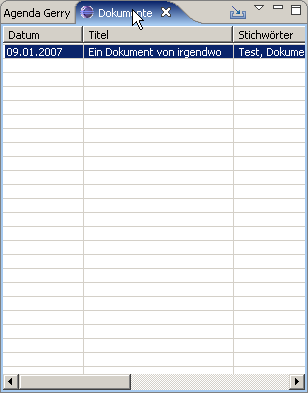
\includegraphics[width=7cm]{images/omnivore1}
% omnivore1.png: 308x393 pixel, 96dpi, 8.15x10.40 cm, bb=0 0 231 295
\end{wrapfigure}

La méthode par omnivore a l'avantage de laisser tous les documents dans le format original. Ceci apporte par contre le désavantage que ces documents ne peuvent être lus qu'avec les programmes appropriés. Si vous sauvegardez ici par exemple des documents en format pdf,il vous faut pour les voir un Acrobat Reader ou un autre programme compatible. Si vous prenez en considération ceci le travail avec omnivore devient très facile:\\
\medskip
Veuillez ouvrir la View documents omnivore:
Vous y trouvez un tableau avec tous les documents qui avaient été attribués au patient choisi. Vous pouvez ajouter à la liste un nouveau document en utilisant glisser-déposer pour le laisser \textit{tomber} dans la liste ou en cliquant le bouton d'importation à droite en haut. Ceci ouvre un dialogue dans lequel vous pouvez introduire un titre et des mots clés concernant le document à importer.

Vous pouvez ouvrir par double-clic un document qui avait été importé. Ceci ne fonctionne par contre seulement (comme déjà mentionné) si dans le système d'exploitation le type de ce fichier s'ouvre avec un programme qui y est installé. 

En cliquant sur la touche droite de la souris étant sur un document vous allez trouver un menu contextuel par lequel vous pouvez changer les informations concernant le document. Il s'y trouve aussi la possibilité d'effacer le document.  
Tout document qui avait été importé de cette manière sera sauvegardé dans la base de données de Elexis. Vous n'avez donc plus besoin de garder le document original. Après l'importation le document ne peut plus être changé. (Si vous l'ouvrez par la suite pour y faire des changements, le document restra pourtant en forme de l'original dans la base de données. La seule chose que vous pourriez faire c'est de l'effacer et le réimporter.).



